\subsection{}
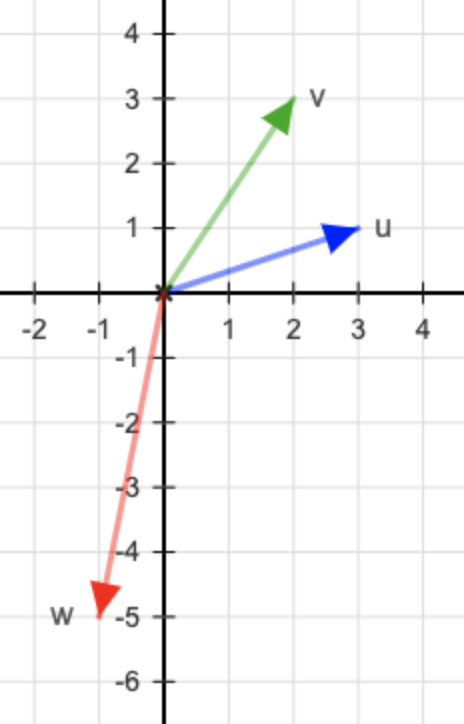
\includegraphics[scale=0.4]{uppg1_1}
\begin{enumerate}
	\item[a)]
	      .\\
	      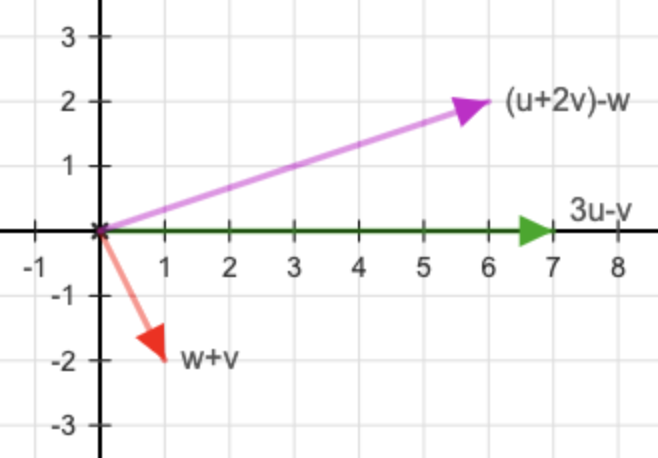
\includegraphics[scale=0.4]{uppg1_1_a}
	\item[b)]
	      .\\
	      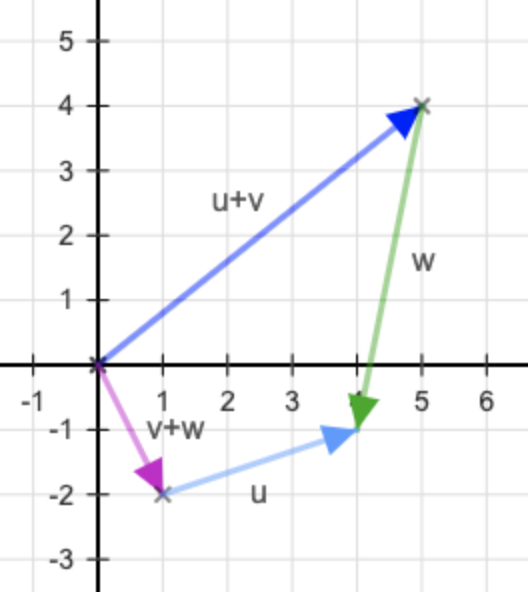
\includegraphics[scale=0.4]{uppg1_1_b}
	\item[c)]
	      \begin{math}
	      	u=
	      	\begin{pmatrix}
	      		3 \\
	      		1 
	      	\end{pmatrix},
			\hspace{6px}
	    	v=
	      	\begin{pmatrix}
	      		2 \\
	      		3 
	      	\end{pmatrix},
			\hspace{6px}
	      	w=
	      	\begin{pmatrix}
	      		-1 \\
	      		-5 
	      	\end{pmatrix}\\
	      	w=su+tv\\
	      	\begin{pmatrix}
	      		-1 \\
	      		-5 
	      	\end{pmatrix}
	      	=s
	      	\begin{pmatrix}
	      		3 \\
	      		1 
	      	\end{pmatrix}
	      	+t
	      	\begin{pmatrix}
	      		2 \\
	      		3 
	      	\end{pmatrix}\\
	      	\begin{cases}
	      		-1=3s+2t \\
	      		-5=s+3t  
	      	\end{cases}\\
	      	(3s+2t)-3(s+3t)=(-1)-3(-5)\\
	      	3s+2t-3s-9t=14\\
	      	-7t=14\\
	      	t=-2\\
	      	s=(-5)-(3t)=(-5)-(-6)=1\\
	      	\begin{cases}
	      		s=1  \\
	      		t=-2 
	      	\end{cases}\\
	      	w=u-2v
	      \end{math}
\end{enumerate}